\chapter{LoRa and LoRaWAN}
\label{chap:lora_and_lorawan}
LoRa is a modulation technique derived from chirp
spread spectrum technology\cite{what_is_lora}. 
Originally developed by Cycleo, a french company, LoRa has been acquired by Semtech~\cite{limits_lora}.
LoRa signals spread over multiple frequencies using the whole available bandwidth.
This makes the signal more resilient against noise on a disrupting frequency. As LoRa
signals are sent over the unlicensed ISM bands, this resilience is an important factor.
While LoRa is the modulation technique on the physical layer, LoRaWAN on the other hand 
is an open communication protocol backed by the Lora Alliance. LoRaWAN specifies packet format,
duty cycles, key exchanges and many more things needed for an efficient and cooperative LoRa network.
A LoRa network is a LPWAN where battery powered devices can stay operating up to 17 years, making LoRa
a popular choice for IoT devices as shown in the example given in the introduction in chapter~\ref{thesis:introduction}. 
The TTN network for example is used for cattle tracking, smart irrigation as well as smart parking applications~\cite{ttn}.

\begin{figure}[h]
    \centering
    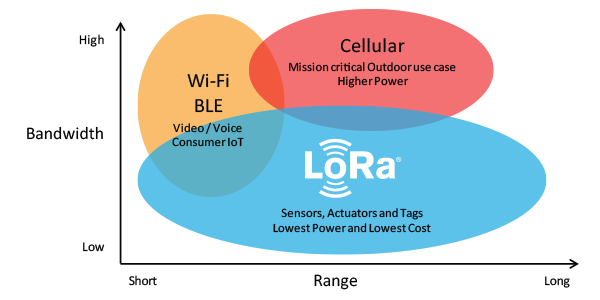
\includegraphics[width=1\textwidth]{figures/LoRa_context.png}
    \caption{LoRa vs other wireless technology\cite{lora_context}}
    \label{fig:lora_context}
\end{figure}

Figure~\ref{fig:lora_context} shows LoRa compared two other wireless technologies, Wi-Fi and cellular. Both Wi-Fi and cellular
are high in bandwidth with cellular having a longer range than Wi-Fi. They both have a much higher power consumption compared to LoRa.
LoRa has lower bandwidth but a high range. In an experiment during a TTN conference, LoRa signals from a low orbit satellite were received~\cite{loa_satellite}.
On the other hand, as LoRa is designed for long-range and low power, only few bytes are transmitted per day while Wi-Fi and cellular are capable of video streaming.
In urban areas LoRa has a range of 2-5 km and 15 km in suburban areas~\cite{limits_lora}.\\
LoRaWAN is not the same all around the world. There are regional parameters that come into play, one is for example the frequency band.
In Europe LoRaWAN operates on the in the 863-870MHz and 433MHz ISM band and in North America the 902-928MHz ISM band. Also channel bandwidth and maximum transmission 
settings are regulated by the government and thus are not the same for all regions~\cite{lora_wan_regional}.

\section{LoRaWAN Architecture}
A LoRaWAN network architecture is a star-of-stars topology. The gateways relay the messages between the end-devices and a central network server.
Gateways are connected to the network server via IP connections, converting the RF packets to IP packets and vice versa~\cite{about_lora_wan}.
Network nodes are not associated with a specific gateway, rather messages sent by a node can be received by multiple gateways. Each gateway will then 
forward the message to the network server which does the complex things such as filtering redundant packages, security checks, forwarding the messages
to the right application server etc.~\cite{what_is_lora_wan}.
As network communication is bidirectional, the network server is also responsible for scheduling responses to the end-nodes. There are different classes of 
end-nodes which will be described in the next section.

\begin{figure}[h]
    \centering
    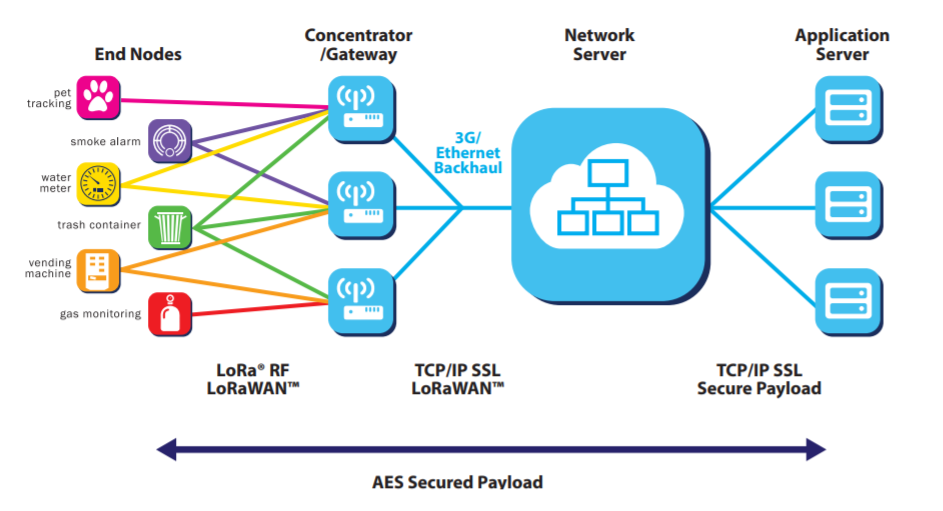
\includegraphics[width=1\textwidth]{figures/lorawan_network.png}
    \caption{LoRaWAN network architecture~\cite{what_is_lora_wan}}
    \label{fig:lorawan_network}
\end{figure}

As depicted in Figure~\ref{fig:lorawan_network}, the packets sent by end-devices (on the far left) such as alarms, tracking devices and monitoring devices,
can be received by multiple gateways. As the end-nodes are not linked to a particular gateway, the can be moved freely which is an important requirement for 
asset tracking.\\
The Figure also shows how security is built into LoRaWAN. The payload is end-to-end encrypted from the end-nodes to the applications server.
A unique 128-bit network session key is shared between the end-device and the network server and 
another 128-bit application session key is shared end-to-end at the application level~\cite{about_lora_wan}.
With those measures LoRaWAN prevents eavesdropping. Spoofing is prevented by a MIC (Message Integrity Code)
in the MAC payload, and replay attacks are prevented by utilizing frame counters~\cite{lora_security}.

\section{End-node Classes}
There are three classes of end-devices. The following description is adapted from the LoRa Alliance guide~\cite{about_lora_wan,what_is_lora}:
\begin{itemize}
    \item Class A, Lowest power, bi-directional end-devices:\\
    \\
    This is the default class, supported by all LoRaWAN devices.
    It is always the end-node that initiates the communication. After an uplink,
    two downlink windows open for the end-device to receive a response, enabling bi-directional communication.
    Either the first is used, or the second, but not both receive windows.
    The end-device can rest in low-power sleep mode, wake up when it needs to send a packet, receive a response
    in the downlink window, then go back to seep. This is an ALOHA-type of protocol. Class A devices have the lowest 
    power consumption. Downlinks from the server have to wait for an uplink from end-device and cannot be initiated directly.
    \item Class B, Bi-directional end-devices with deterministic downlink latency:\\
    \\ 
    Additionally to Class A receive windows, a Class B device opens extra receive windows at scheduled times.
    This is achieved by time-synchronized beacons from the gateway to the end-device to notify the end-device
    to open a receive window.

    \item Class C, Lowest latency, bi-directional end-devices:\\
    \\
    Devices of this class have always open receive windows, except for when they are themselves transmitting.
    A downlink transmission can be initiated by the network server at any time (assuming the device is not currently transmitting)
    resulting in no latency. Class C devices however use the most energy. They are more suitable for plugged in devices rather than
    battery powered devices.

\end{itemize}

\section{LoRa Signal (Uplink)}

\subsection{Chirps}
A LoRa signal is a series of so called chirps as LoRa is derived from the Chirp Spread Spectrum modulation (CSS) technique. 
There are up-chirps and down-chirps. In CSS chirps are deliberately spread across the available bandwidth. Up-chirps go from low frequency 
to high frequency and down-chirps go from high frequency to low frequency. In Europe the LoRaWAN signal bandwidth is 125 kHz with one exception. Assuming a center
frequency of 868.5 MHz, which is in the European ISM band, a full up-chirp, so called sweep, would go from 868.4375 MHz to 868.5625 MHz.

\begin{figure}[h]
    \centering
    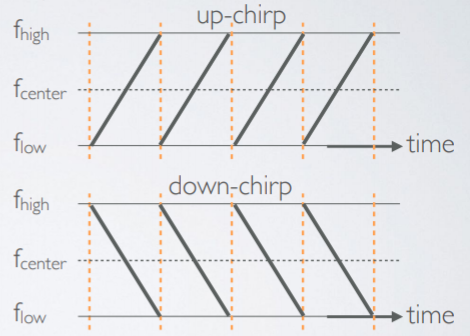
\includegraphics[width=0.6\textwidth]{figures/chirp_mobilefish.png}
    \caption{Up- and down chirps~\cite{lora_chirp_mobilefish}}
    \label{fig:chirp_mobilefish}
\end{figure}

Figure \ref{fig:chirp_mobilefish} shows the linear frequency increase resp. decrease over time over the full bandwidth
for up-chirps and down-chirps. Data is encoded by frequency jumps in the chirps. 

\begin{figure}[h]
    \centering
    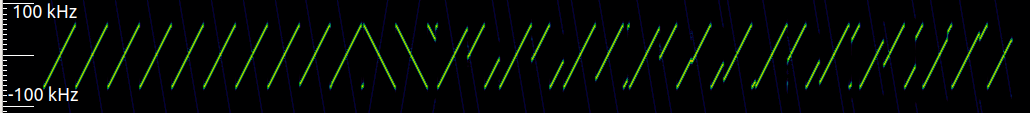
\includegraphics[width=1\textwidth]{figures/signal_Goodbye!_SF9_CR4_5.png}
    \caption{Own recording of uplink transmission by arduino equipped with a LoRa shield}
    \label{fig:Goodbye}
\end{figure}

The LoRa signal shown in~\ref{fig:Goodbye} carries the message  "Goodbye !". This message was sent 
with a spreading factor (SF) of 9 and coding rate of 4/5. The terms spreading factor and coding rate 
will be discussed later on.\\
As one can see, a typical LoRa signal start with a so called preamble, which are the 10 up-chirps at 
the beginning. Those are followed by two down-chirps, which signify the end of the preamble and the start 
of the actual payload. In this payload is a header, the actual encoded message followed by a Cyclic Redundancy Check (CRC).
The CRC is used for error correction.
\subsection{Symbol and Spreading Factor}
A LoRa signal holds various symbols. A symbol encodes one or more bits of data.
The spreading factor determines the number of encoded bits in a symbol.
In the shown recording one symbol holds 9 bits of data as the spreading factor of that signal was set to 9.
It follows that a symbol has $2^{SF}$ values. Those values range from 0 to 511 in case of SF 9. A sweep signal of SF 9
thus has 512 chips (no to be confused with chirps)~\cite{lora_symbol_mobilefish}.
The chips go linearly from low to high and then wrap around, once the maximum frequency is reached.
\\
In Figure~\ref{fig:fict_symbols} a fictional symbol with SF 7 is shown. This particular 
arrangement of chips highlighted in orange would denote the symbol "1011111". Those 7 bits correspond 
to the decimal value 95.
\begin{figure}[h]
    \centering
    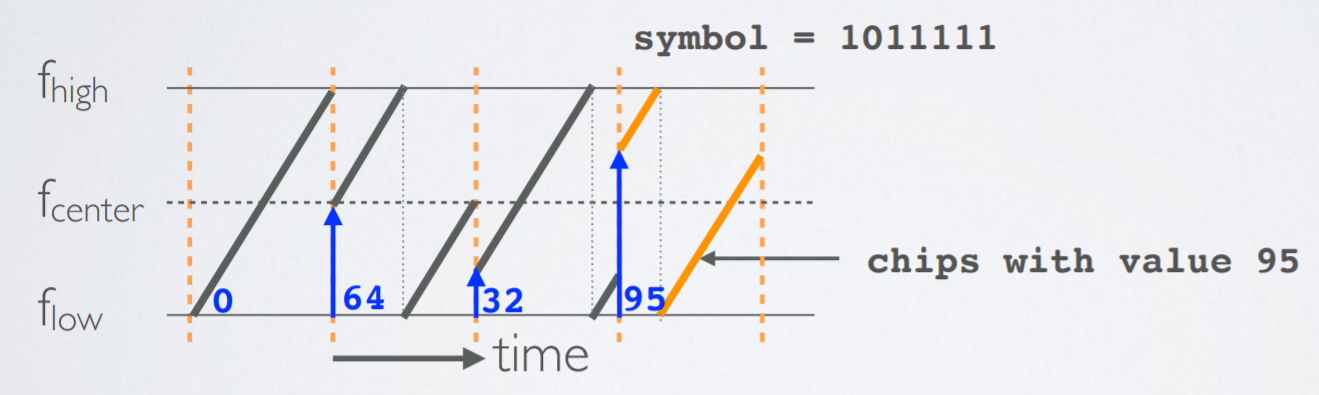
\includegraphics[width=1\textwidth]{figures/chips_and_symbols.png}
    \caption{Chips and symbols value~\cite{lora_symbol_mobilefish}}
    \label{fig:fict_symbols}
\end{figure}

In Figure \ref{fig:Goodbye_decoded}, a real world example is shown. The same LoRa signal as in Figure~\ref{fig:Goodbye} with SF 9 showing the message "Goodbye !"
run through modified version of the LoRa decoder by Robyns et al.~\cite{robyns} and then through a python script where we match the samples to the symbols and their 
values. The last symbol encodes the hex value 142 which corresponds to these 9 bits "101000010". In a SF 9 signal each symbol encodes 9 bits.
\begin{figure}[h]
    \centering
    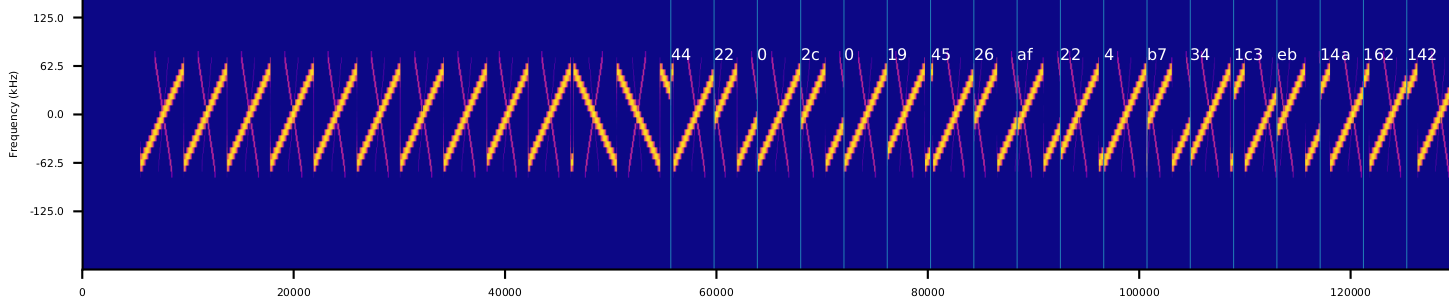
\includegraphics[width=1\textwidth]{figures/Goodbye_decoded.png}
    \caption{Running the signal through our toolchain, matching symbols with samples}
    \label{fig:Goodbye_decoded}
\end{figure}

\subsection{Coding Rate}
LoRa signals are encoded with a coding rate (CR). The CR denotes the proportion of how many bits carry actual information. The bits that do not carry information are used 
for Forward Error Correction. The formula for coding rate is $CR=4/(4 + CR)$ where CR $\in \{1,2,3,4\}$. A CR of 1 is thus the proportion of 4/5 of actual information over 
bits used for error correction\cite{SX_design_guide,coding_rate_mobilefish}.
With FEC, corrupted bits e.g. due to interference, can be corrected. With CR of 4, corresponds to $4/8 = 1/2$, half the transmitted bits carry information, the other half is for FEC.
The higher the CR (from 1-4) the more bits can get corrupted and corrected by FEC.
On the other hand, the higher the CR the more bits need to be transmitted which drains the battery more.

\subsection{Spreading Factor \& Time on Air}
The longer the packet, the longer the transmission time. LoRa packets can be shortened
by sending packets in implicit header mode where
no header is sent and the settings that would have been specified in the header have to be 
predefined manually on the end-device.\\
Assuming constant packet size and same bandwidth, varying the spreading factor increases resp. decreases the time on air.
The higher the SF, the longer the time on air. Higher SF means longer range. The spreading factor goes from 7 to 12. SF 7 has 
the shortest range, SF 12 the longest. The spreading factor essentially sets the duration of a chirp, a full sweep~\cite{exploratory_eng}.
\\
The symbol time is defined in the LoRa Design guide by $T_{sym} = \frac{2^{SF}}{BW}$~\cite{SX_design_guide}.
It follows as stated above, that the higher the SF the longer the symbol duration. Also, the higher the bandwidth (BW) the shorter
the symbol duration. In Europe the BW is 125~kHz, while in North America a BW of 500~kHz is allowed.
It also follows that with an increase in SF by 1 the symbol duration is doubled. The bit rate $R_{b}$  is then defined by 
$R_{b} = SF*\frac{[\frac{4}{4 * CR}]}{[\frac{2^{SF}}{BW}]}$ with CR being the coding rate for the error correction scheme~\cite{lora_modulation_basics}.
It follows from the formula that the higher the coding rate the lower the bit rate, as with a higher CR more redundancy is added 
for the error correction scheme. Highest data rate for $BW=125~kHz$ and $CR=1$ is achieved 
with SF 7 resulting in a data rate of 5.5 kbits/s and the lowest data rate is achieved with SF 12 resulting in a data rate 0.29 kbits/s.
\\
The spreading factors are orthogonal to each other, meaning signals on different spreading factors do not interfere with each other. This is 
Code Division Multiple Access (CDMA) where a shared medium is used and the bandwidth is optimized for multiple access.
\\
To optimize network capacity LoRaWAN employs a method called Adaptive Data Rate (ADR). With ADR the network server signals 
the end-device which spreading factor to use according to some measurements including the signal to noise ratio. Let's assume there are multiple devices near a gateway 
that transmit with SF 12. This occupies the bandwidth for devices that are farther away and actually need SF 12.
The network server detects that the nearby devices do not need a spreading factor of 12 and signal them to use 
a lower SF such as SF 7 or SF 8. The ADR setting has to be enabled on the end-devices and can be disabled.

\subsection{Packet Structure}
\label{sec:pkt_structure}
The base form of a LoRa packet starts with the preamble, followed by the optional header with a header CRC, followed by the payload and finally the 
payload CRC. The number of payload symbols is calculated by the following formula~\cite{SX_design_guide}:\\ \\
$payloadSymbNb = 8 + max{(ceil(\frac{8PL-4SF+28+16-20H}{4(SF-2DE)})*(CR+4),0)}$ 
\\ \\

\begin{figure}[h]
    \centering
    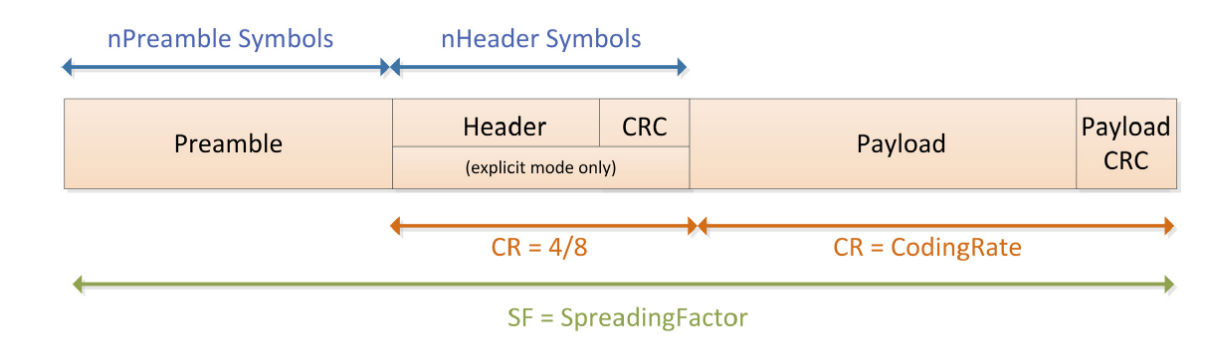
\includegraphics[width=1\textwidth]{figures/packet_struct.png}
    \caption{LoRa packet structure~\cite{SX_design_guide}}
    \label{fig:packet_struct}
\end{figure}

With: 
\begin{enumerate}
    \item PL being the number of payload bytes
    \item SF being the spreading factor
    \item H = 0 if header is enabled and H = 1 if no header
    \item DE = 0 if low data rate optimization is enabled and DE = 0 if disabled
    \item CR being the coding rate
    
\end{enumerate}

As Figure~\ref{fig:packet_struct} shows, the header is always encoded with the highest coding rate, $CR=4$.
This is because the header contains crucial information such as the packet length.

Figure \ref{fig:uplink_struct} shows the structure of an uplink packet. PHDR stands for PHY header.
Those are "raw" LoRa packets. LoRaWAN packets have additional fields such as MAC header (MHDR) and 
frame header (FHDR). Those are all in PHY payload of the "raw LoRa" packet as Figure~\ref{fig:lora_wan_struct} 
shows.   
\begin{figure}[h]
    \centering
    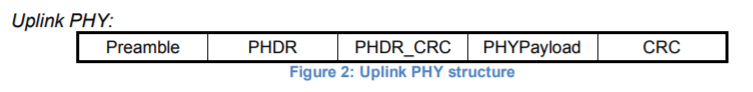
\includegraphics[width=1\textwidth]{figures/uplink_struct.png}
    \caption{LoRa uplink packet structure~\cite{lora_wan_spec}}
    \label{fig:uplink_struct}
\end{figure}


\begin{figure}[h]
    \centering
    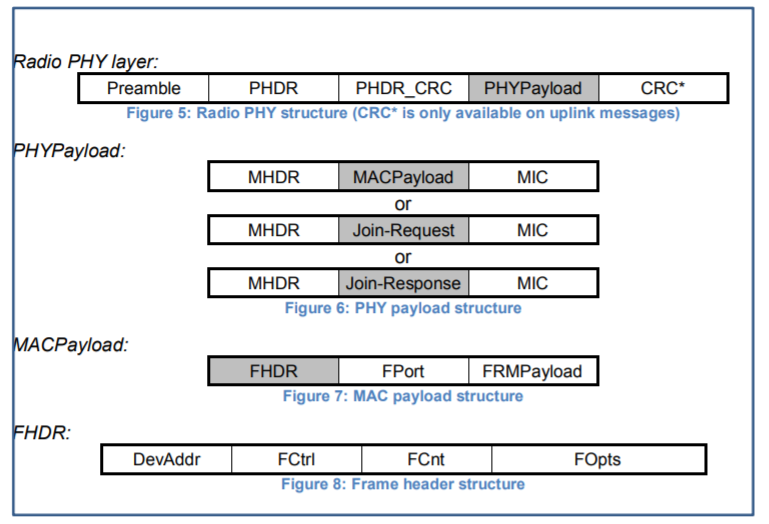
\includegraphics[width=1\textwidth]{figures/lorawan_struct.png}
    \caption{LoRaWAN packet~\cite{lora_wan_spec}}
    \label{fig:lora_wan_struct}
\end{figure}

\section{LoRa Signal (Downlink)}
LoRa downlinks signals are the inverse of an uplink signal. 
This lets end-devices or gateways easily differentiate between uplink and downlink.
An Arduino end-device can then ignore all uplink signals as it will only ever expect a downlink signal it may need to process.
Gateways on the other hand can ignore downlink signals as they are only interested in uplink signals.
Figure~\ref{fig:lora_down_sig} shows a downlink signal with SF 12 and coding rate 4/5 sent from LoRa gateway. It encodes the payload "ACK".
\begin{figure}[h]
    \centering
    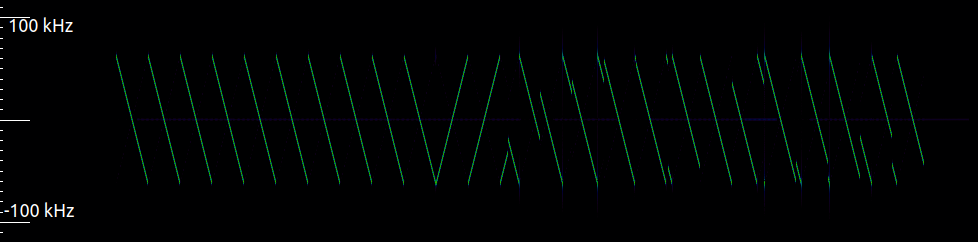
\includegraphics[width=1\textwidth]{figures/down_ack_sf_12_cr_4_5.png}
    \caption{LoRaWAN packet~\cite{lora_wan_spec}}
    \label{fig:lora_down_sig}
\end{figure}
A difference is that downlinks signals 
do not have a CRC after the payload as shown in Figure\ref{fig:downlink_struct}.

\begin{figure}[h]
    \centering
    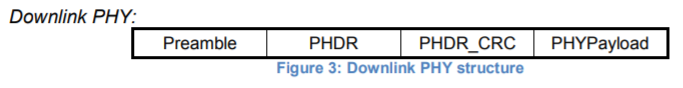
\includegraphics[width=1\textwidth]{figures/downlink_struct.png}
    \caption{LoRa downlink packet structure~\cite{lora_wan_spec}}
    \label{fig:downlink_struct}
\end{figure}

The 10 preamble chirps that are up chirps in an uplink signal are now down chirps.
\newpage
The 2 start of frame delimiter chirps that are down chirps in an  uplink signal are now up chirps.
The question remains if the data chirps are flipped as well. In fact, the data chirps are flipped as well, 
as we have discovered. This will be elaborated on more in chapter~\ref{chap:lora_tools}.


\chapter{LoRa in SDRs}
Software-defined radios (SDR) use components that are usually implemented in hardware.
The most popular signal processing framework is GNU Radio.
For LoRa we were looking for an existing implementation that demodulates, and also modulates LoRa signals.

\section{Existing Implementations}
There are three existing implementations we looked at:
\begin{itemize}
    \item Josh Blum's LoRa Mod -and Demodulator for LoRa in the Pothos framework \url{https://myriadrf.org/news/lora-modem-limesdr/}
    \item Matt Knight's GNU Radio Module \url{https://github.com/BastilleResearch/gr-lora}
    \item Robyns et al. LoRa Module for GNU Radio \url{https://github.com/rpp0/gr-lora}
\end{itemize}

We tried Blum's implementation in the Pothos first. The Pothos projects is an open source data-flow framework
supporting SoapySDR, a general framework for enabling SDR devices~\cite{pothos}.
Unfortunately the LoRa modem demo application did not work for us at all. After spending a few unsuccessful days 
trying to get to the issue we moved to Knight's application.

Matt Knight held a great talk on reverse engineering LoRa at the GNU Radio conference 2016 \url{https://www.youtube.com/watch?v=-YNMRZC6v1s}.
GNU Radio, as Pothos, is a framework for signal processing.\\
From the GNU Radio website:
\begin{displayquote}
    GNU Radio is a free \& open-source software development toolkit that provides signal processing
    blocks to implement software radios. It can be used with readily-available low-cost external
    RF hardware to create software-defined radios, or without hardware in a simulation-like environment.
    It is widely used in research, industry, academia, government, and hobbyist environments to support both wireless
    communications research and real-world radio systems.~\cite{gnuradio}
\end{displayquote}

GNU Radio already comes with a wide set of blocks. Extensions are called Out Of Tree modules (OOT) as they are not in the 
standard tree of blocks. Knight's implementation did not work well for us. If we got an output from the decoder, it was not 
what was expected. A reason could be that in his examples the signal source block is an USRP SDR while we had a LimeSDR mini 
at our disposal. Simply switching the source blocks probably is not enough. We did not investigate the compatibility between LimeSDR mini
and and USRP further but moved on to the final implementation.
His blocks are in modular fashion. The demodulator and decoder are separate blocks. Channelization and fine tuning must be done 
explicitly before passing the stream to the demodulator block.

\begin{figure}[h]
    \centering
    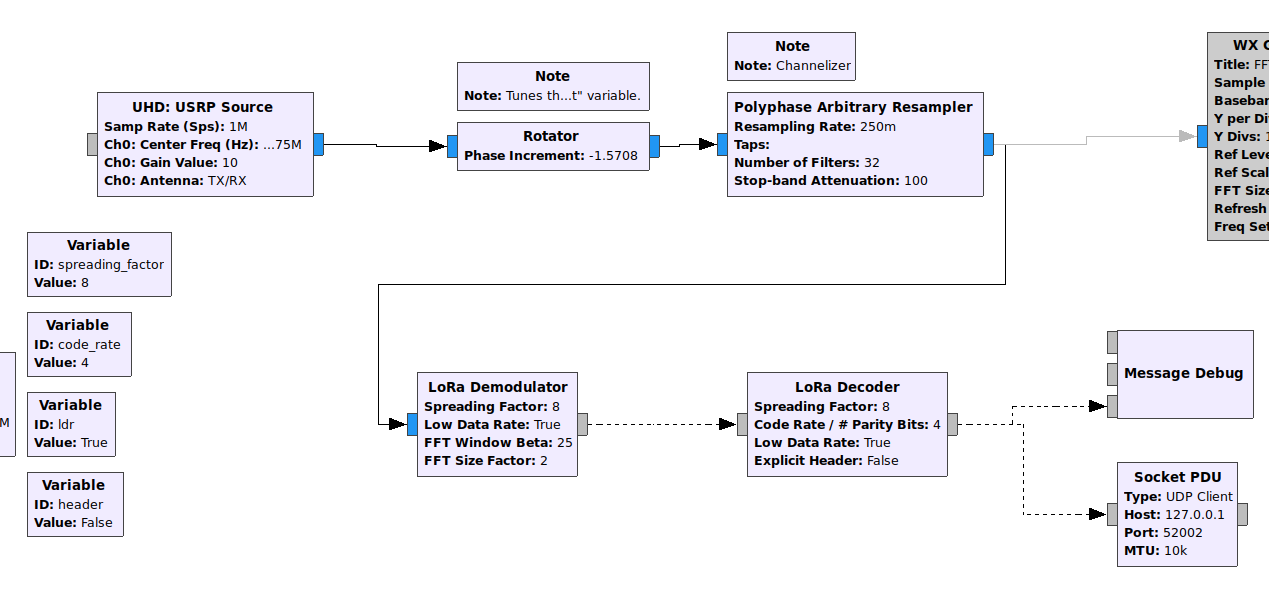
\includegraphics[width=1\textwidth]{figures/matt_gnu_example.png}
    \caption{Knight's GNU Radio gr-lora OOT RX example~\cite{knight_implementation}}
    \label{fig:knight_gnu}
\end{figure}

Figure~\ref{fig:knight_gnu} shows the typical flow of a GNU Radio flowgraph where data is passed 
from block to block as a stream (blue connection ports) or as message blocks (grey connection ports).
\\
Robyns' implementation is also an OOT module for GNU Radio. It has an elaborate 
installation and usage guide. A docker environment is also provided for testing the 
decoding of a LoRa signal, which is a big plus. Unlike Knight's implementation, this module
has demodulation, decoding and channelization all in one single block as shown in Figure~\ref{fig:robyns_gnu}. 
The module has been tested with various SDR devices but not with the LimeSDR mini. Nevertheless it worked
well for us and we based the C-RAN implementation for LoRa on this module.

\begin{figure}[h]
    \centering
    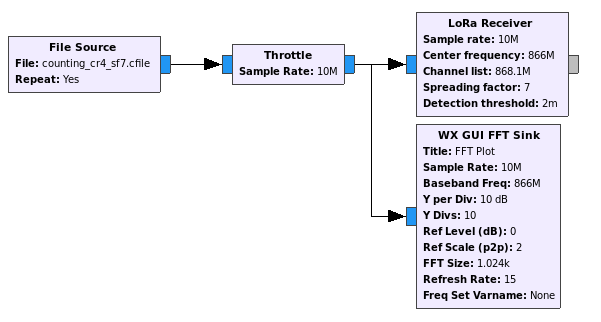
\includegraphics[width=0.8\textwidth]{figures/robyns_gnu.png}
    \caption{Single LoRa Receiver block (top right)~\cite{robyns_implementation}}
    \label{fig:robyns_gnu}
\end{figure}

\section{LoRa Decoding}
The difficulty with reverse engineering LoRa is that its proprietary and
there is no official documentation on the PHY. To reverse engineer, information hints
on the PHY layer have to be taken from various official LoRaWAN documents, from patents, and the 
rest is guesswork. To make it more difficult, some of the documentation is a lie as the PHY is not implemented 
in the way it is described, see Knight~\cite{knight_youtube}. 
The data is encoded before it is sent over the air to make it more resistant against interference.
Thus after demodulating the signal with a Fourier Transform, the data has to be decoded to make it usable.
Semtech's European patent hints at the following four steps:
\begin{enumerate}
    \item Symbol gray indexing. This adds error tolerance.
    \item Data whitening. This induces randomness.
    \item Interleaving. This scrambles the bits within a frame.
    \item Forward Error Correction. This adds correction parity bits.
    
\end{enumerate}
Those are 4 distinct operations which have to be reverse engineered~\cite{knight_youtube}.\\
Robyns et al. identified and implemented the following seven steps in their receiver to 
receive and decode a LoRa signal: detection, synchronization, demodulation, deinterleaving, dewhitening,
decoding, and packet construction~\cite{robyns_implementation}. They also provide a detailed description of the 
packet structure, especially the header. They deduce that because the minimum SF is SF 7, and the header is always 
transmitted mit CR = 4, it must fit in an interleaving matrix of a certain size which results in the header heaving a size of 
40 bits. The header contains important data as the payload length, thus it makes sense that the header is always sent with the highest
coding rate.
At the time of Knight's talk, he did not decode the header. Robyns implementation is quite complete except for CRC checks of the payload and header
as well as decoding multiple channels simultaneously. 

\chapter{C-RAN in Cellular Networks}
\label{chap:cran_in_cellular}
A Radio Access Network (RAN) provides the connection between and end-device e.g. a mobile phone and the core network e.g network of the telecom provider.
A RAN provides access and manages resources across the radio sites. It is a major component in telecommunications. RAN components include a base station and antennas
that cover a specific region. The base stations connect to the core network~\cite{what_is_ran}.

\section{D-RAN}
Distributed Radio Access Network (D-RAN) is the present mode of operation for many mobile network operators.
In a D-RAN, the 4G radio at the site tower consists of a Baseband Unit (BBU) on the ground and a Remote Radio Head (RRH)
at the top as Figure~\ref{fig:DRAN} shows. RRH and BBU are connected via the Common Protocol Radio Interface (CPRI).
The BBUs in each tower are connected via ethernet to the Mobile Switching Center (MSC)~\cite{fujitsu}. 

\section{Moving to C-RAN}
\label{sec:moving_to_cran}

\begin{figure}[h]
    \centering
    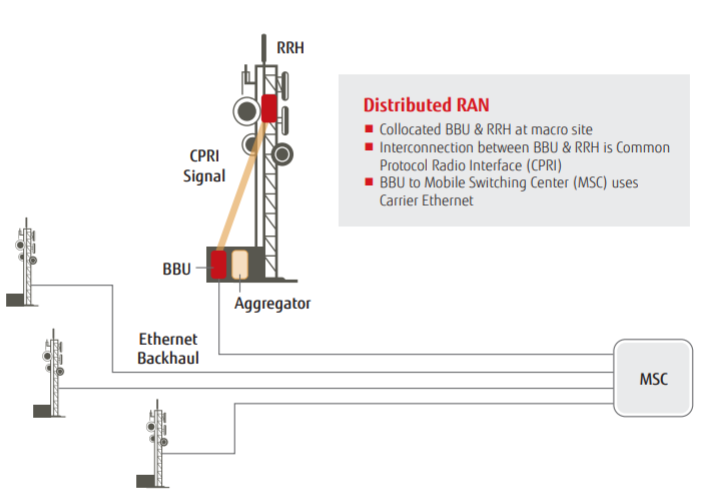
\includegraphics[width=1\textwidth]{figures/DRAN.png}
    \caption{Distributed cell towers with each with a RRH and BBU~\cite{fujitsu}}
    \label{fig:DRAN}
\end{figure}

In a Cloud / Centralized RAN (C-RAN) the BBU in each tower site are move into a centralized place, the BBU hotel, see Figure~\ref{fig:CRAN}.
This new architectural setup results in saving costs in capital expenditures (CAPEX) as well as operational expenditures (OPEX). The many small routers in the cell towers
can be replaced by one in the BBU hotel. Deployment, maintenance and scaling can be expedited as all the BBU are centralized.
Also this enables the BBU for Network Function Virtualization (NFV) and the RAN for Software Defined Networking (SDN)~\cite{fujitsu}.

\begin{figure}[h]
    \centering
    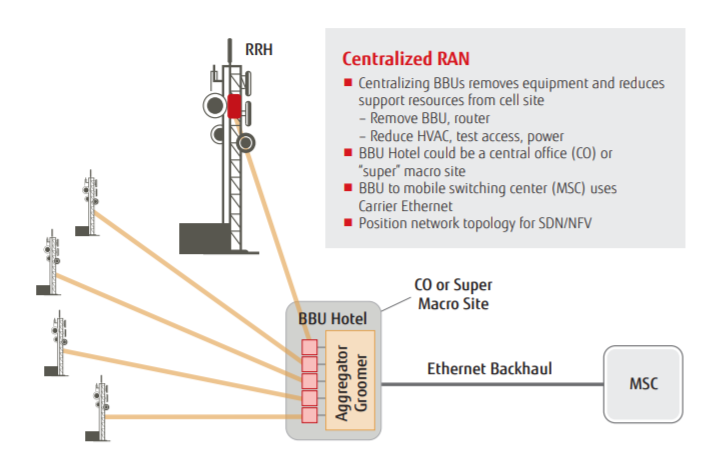
\includegraphics[width=1\textwidth]{figures/CRAN.png}
    \caption{BBUs are centralized in the BBU hotel~\cite{fujitsu}}
    \label{fig:CRAN}
\end{figure}

\section{Virtual RAN}
In virtual RAN the execution environment is abstracted i.e. virtualized.
Radio function applications operate in a virtualized environment and interact
with physical resources directly or through hardware emulation.
Such a cloud environment enables RAN as a service~\cite{Nikaein2015}.
For C-RAN this means instead of having a separate standalone physical device
for each BBU in the BBU hotel, the BBUs now can run on a single physical server with each
BBU in a virtualized environment. \\
Nikaein et al. describe two main steps for realizing a C-RAN namely:
\begin{itemize}
    \item \textbf{Commoditization and Softwarization} which essentially is the implementation of network and RF function in software.
    \item \textbf{Virtualization and Cloudification} which is the execution of network functions and management of physical resources by a cloud OS~\cite{Nikaein2015}.
\end{itemize}

Nikaein et al. found that containers e.g. Docker proved to be more adequate in their RAN as a service experiment as they offer near bare metal performance
and provide direct access to the RF hardware. Virtual machines in, particular KVM, also gave them good performance, but require low latency mechanisms to access I/O resources.
\\
For the C-RAN for LoRa, described in chapter~\ref{chap:cran_for_lora}, Docker is used for the virtualization layer.
